\begingroup
\setlength{\parindent}{0pt}
\setlength{\parskip}{0.24em}
\setlist[itemize]{leftmargin=1.05em,itemsep=0.16em,topsep=0.12em,parsep=0em}

\definecolor{cardborder}{HTML}{BFC4C9}
\definecolor{headerbg}{HTML}{F1F3F4}
\definecolor{summarybg}{HTML}{FFF7E6}
\definecolor{inputbg}{HTML}{EDF7F6}
\definecolor{evalbg}{HTML}{EEF6EA}
\definecolor{softwarebg}{HTML}{F6F6F8}
\definecolor{analysisbg}{HTML}{FCEDEA}
\definecolor{failbg}{HTML}{FBEDEA}
\definecolor{failred}{HTML}{A83A33}
\definecolor{partialbg}{HTML}{FFF2D5}
\definecolor{partialorange}{HTML}{855A00}
\definecolor{successbg}{HTML}{EAF5EC}
\definecolor{successgreen}{HTML}{2F6F3E}

\newcommand{\Code}[1]{\texttt{\detokenize{#1}}}
\newcommand{\Chip}[1]{\begingroup\setlength{\fboxsep}{2pt}\colorbox{headerbg}{\scriptsize #1}\endgroup}
\newcommand{\StatusBadge}[3]{\begingroup\setlength{\fboxsep}{3pt}\colorbox{#2}{\textcolor{#3}{\textbf{#1}}}\endgroup}
\newcommand{\BlockTitle}[1]{{\raggedright\textbf{\footnotesize #1}\par}\vspace{2pt}}

\newtcolorbox{ColorTaskCard}[1]{
  enhanced,
  colback=white,
  colframe=cardborder,
  boxrule=0.8pt,
  arc=0pt,
  left=7pt,
  right=7pt,
  top=6pt,
  bottom=7pt,
  before skip=0.25em,
  after skip=0.25em,
  title={#1},
  coltitle=black,
  colbacktitle=headerbg,
  fonttitle=\bfseries\large
}

\newtcolorbox{CardBlock}[3][]{
  enhanced,
  colback=#2,
  colframe=#3,
  boxrule=0.25pt,
  arc=1pt,
  left=7pt,
  right=7pt,
  top=5pt,
  bottom=5pt,
  before skip=4pt,
  after skip=4pt,
  before upper={\scriptsize\raggedright},
  #1
}

\subsubsection{Representative Task Cards}
\label{app:representative-gui-task-cards}
\small
We present representative task cards to illustrate how ALE task instances are specified, executed,
and scored. Each card summarizes the agent-facing request, input materials, expected deliverables,
evaluation rubric, observed score, and observed outcome for one executed task instance. All trajectories
shown here were produced by the Claude Code harness running Claude Opus 4.7. These cards
are intended to make the benchmark construction and evaluation protocol concrete at the instance
level, complementing the aggregate coverage and performance results reported in the main text.
\clearpage
\begin{ColorTaskCard}{Task Card 1: Injection Mold-Flow Analysis \hfill \StatusBadge{PARTIAL}{partialbg}{partialorange}}
\scriptsize
{\textbf{Task ID:} \Code{manufacturing/mold-flow}}\\[-1pt]
{\textbf{Observed score:} 0.476}\quad
\Chip{Manufacturing} \Chip{Moldex3D} \Chip{CAE}

\begin{CardBlock}{summarybg}{summarybg}
\BlockTitle{TASK DESCRIPTION}
Injection mold-flow simulation supports tooling and process decisions. The task provides a meshed Moldex3D project, a process specification, and a results template. The agent must open project 230057, apply process\_spec.json, run fill, pack, cooling, and warp analysis, and write output/results.json with solver-derived pressure, force, time, volume, and weight values.
\end{CardBlock}

\begin{CardBlock}{softwarebg}{softwarebg}
\BlockTitle{SOFTWARE / EXECUTION VIEW}
\centering
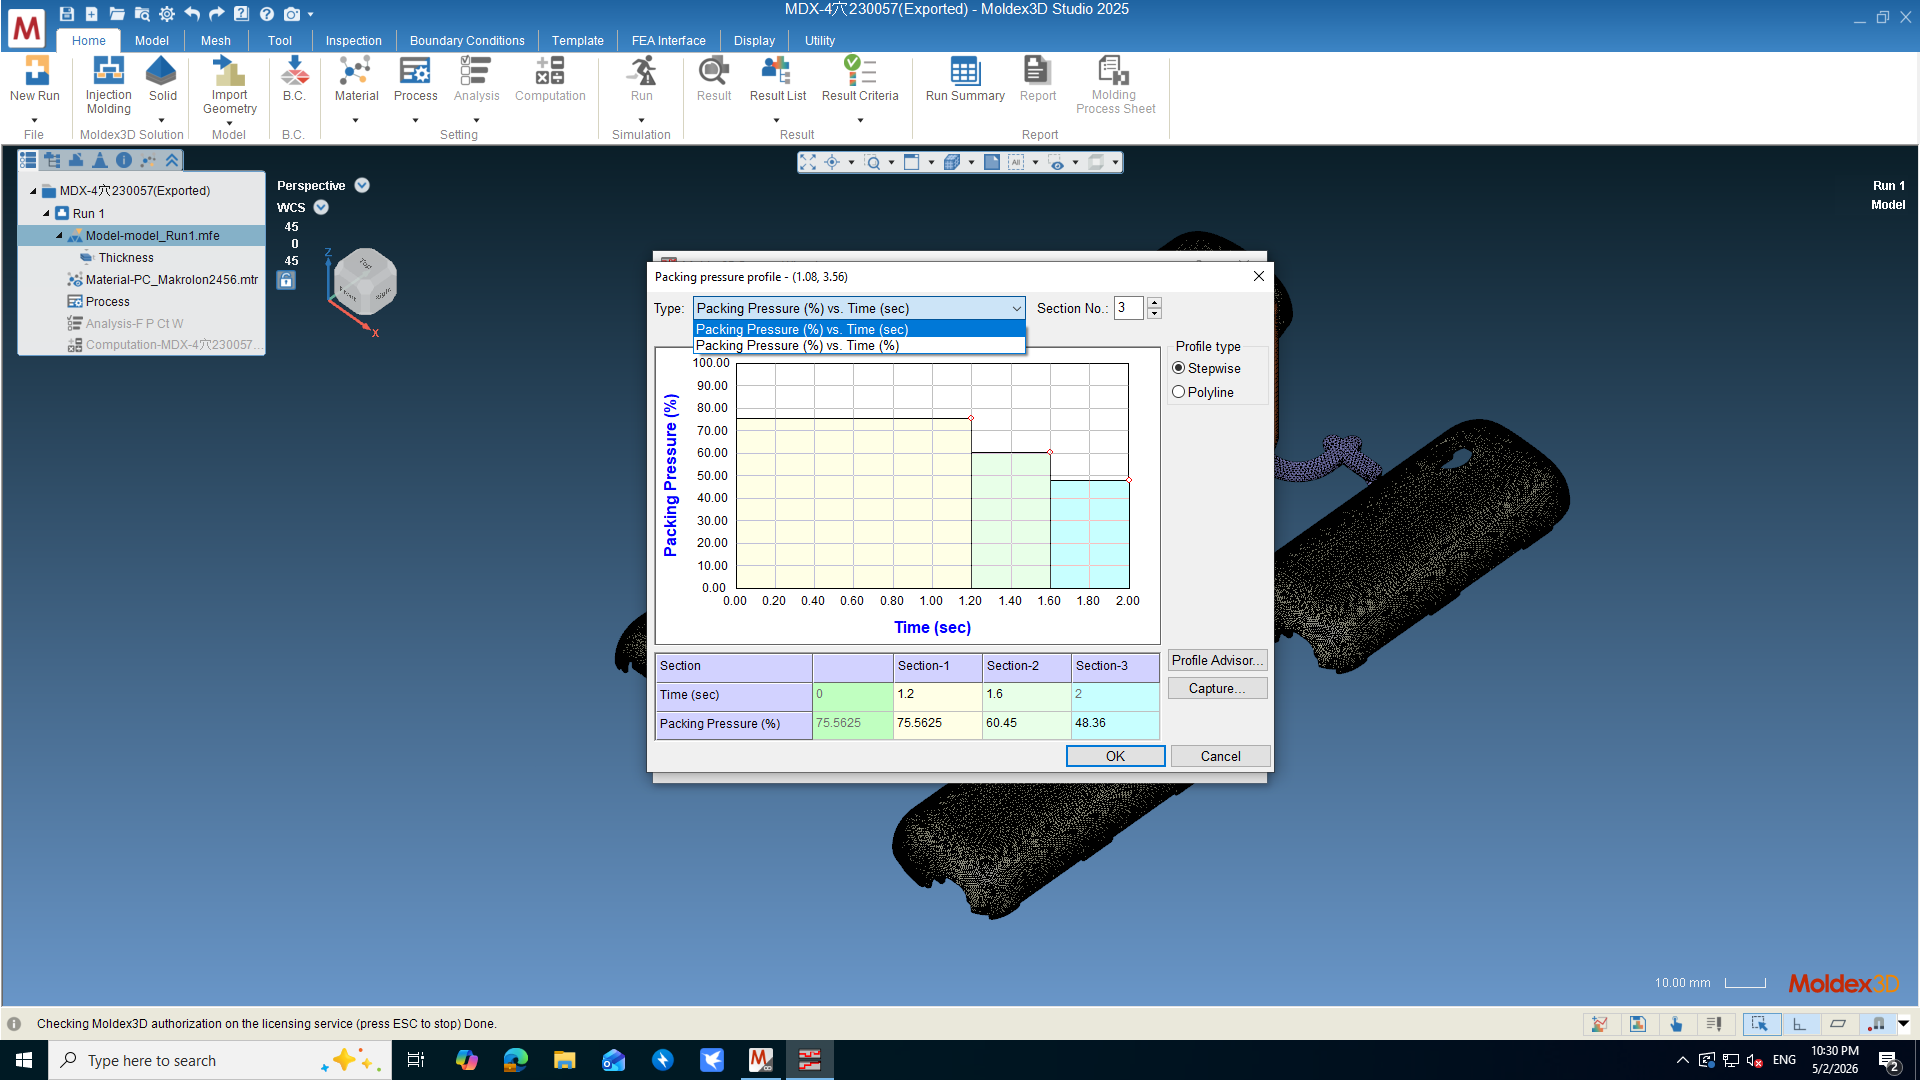
\includegraphics[width=0.985\linewidth,height=3.18in,keepaspectratio]{figures/task-card-assets/gui-economic/manufacturing-mold-flow-execution.png}

\vspace{1pt}
{\scriptsize Moldex3D CAE workflow: the agent is editing the packing-pressure curve for a four-cavity injection-mold simulation. This is the process-setup stage; scoring depends on completing the solver run and extracting the pressure, force, cycle-time, volume, and weight metrics into results.json.}
\end{CardBlock}

\begin{minipage}[t]{0.49\linewidth}
\vspace{0pt}
\begin{CardBlock}{inputbg}{inputbg}
\BlockTitle{INPUT MATERIALS}
\begin{itemize}
\item Staged Moldex3D project with mesh, material, and four-cavity geometry.
\item process\_spec.json specifying fill, pack, cool, and warp process settings.
\item results\_template.json defining every metric required in the final JSON.
\end{itemize}
\end{CardBlock}

\begin{CardBlock}{inputbg}{inputbg}
\BlockTitle{REFERENCE OUTPUT}
\begin{itemize}
\item Saved Moldex3D project after the configured simulation run.
\item output/results.json populated with injection pressure, V/P switch pressure, clamp force, cooling/cycle times, volume, and weight fields.
\end{itemize}
\end{CardBlock}

\end{minipage}\hfill
\begin{minipage}[t]{0.49\linewidth}
\vspace{0pt}
\begin{CardBlock}{evalbg}{evalbg}
\BlockTitle{EVALUATION RUBRIC}
\begin{itemize}
\item Hard gates reject missing, malformed, or all-null results.json.
\item The main score compares each numeric field with a hidden solver reference within 1 percent relative tolerance.
\item Generated project artifacts can provide limited partial credit only when the main metrics are weak.
\end{itemize}
\end{CardBlock}

\begin{CardBlock}{analysisbg}{analysisbg}
\BlockTitle{OBSERVED OUTCOME}
\begin{itemize}
\item Score: 0.4762. The agent reached the right Moldex3D setup workflow and submitted results.json, but the score indicates only partial numeric/result credit.
\item Failure mode: the submitted metrics were not reliably extracted from completed solver outputs; some values were estimated rather than measured CAE results.
\item Interpretation: successful GUI setup was insufficient without closed-loop numerical verification: wait for result files, inspect or export solver data, then populate the JSON.
\end{itemize}
\end{CardBlock}
\end{minipage}
\end{ColorTaskCard}
\clearpage
\begin{ColorTaskCard}{Task Card 2: Orchestral Music Transcription \hfill \StatusBadge{FAIL}{failbg}{failred}}
\scriptsize
{\textbf{Task ID:} \Code{audio/music_transcription}}\\[-1pt]
{\textbf{Observed score:} 0.000}\quad
\Chip{Audio production} \Chip{Notation} \Chip{Dorico}

\begin{CardBlock}{summarybg}{summarybg}
\BlockTitle{TASK DESCRIPTION}
Orchestral transcription converts an audio recording into a printable score and multitrack MIDI. The task provides an audio brief, a Dorico environment, a named piece, tempo, instrumentation contract, and exact output-file requirements. The agent must follow the Dorico Prelude / Akinola / tempo 140 / 27-instrument specification and deliver transcription.pdf, transcription.mid, and overview.png.
\end{CardBlock}

\begin{CardBlock}{softwarebg}{softwarebg}
\BlockTitle{SOFTWARE / EXECUTION VIEW}
\centering
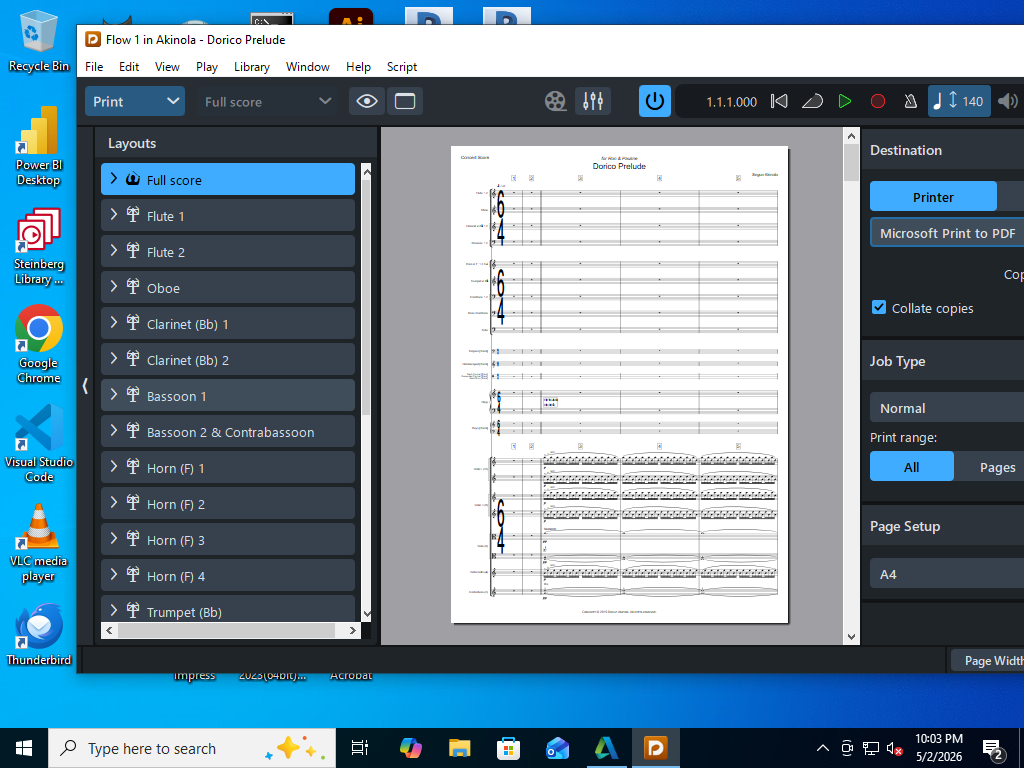
\includegraphics[width=0.985\linewidth,height=3.45in,keepaspectratio]{figures/task-card-assets/gui-economic/audio-music-transcription-execution.png}

\vspace{1pt}
{\scriptsize Music-engraving workflow: Dorico is open on an orchestral score in print/export mode. The task required converting the audio brief into a readable full score and MIDI, then exporting the PDF, MIDI, and overview screenshot to the exact output paths.}
\end{CardBlock}

\begin{minipage}[t]{0.49\linewidth}
\vspace{0pt}
\begin{CardBlock}{inputbg}{inputbg}
\BlockTitle{INPUT MATERIALS}
\begin{itemize}
\item Audio reference and task\_brief.json with title, composer, tempo, instruments, and GM programs.
\item Dorico environment for score engraving and export.
\item Output-path requirements for PDF, MIDI, and overview screenshot.
\end{itemize}
\end{CardBlock}

\begin{CardBlock}{inputbg}{inputbg}
\BlockTitle{REFERENCE OUTPUT}
\begin{itemize}
\item transcription.pdf showing a complete, readable full score.
\item transcription.mid with multitrack timing, pitches, dynamics, and GM Program Change assignments.
\item overview.png showing a notation UI with the produced score.
\end{itemize}
\end{CardBlock}

\end{minipage}\hfill
\begin{minipage}[t]{0.49\linewidth}
\vspace{0pt}
\begin{CardBlock}{evalbg}{evalbg}
\BlockTitle{EVALUATION RUBRIC}
\begin{itemize}
\item Missing PDF, missing MIDI, or missing/invalid notation screenshot triggers a hard zero.
\item After the gates pass, pitch and rhythm each contribute 30 percent, dynamics 20 percent, instrument assignment 10 percent, and score layout 10 percent.
\item The MIDI is compared to a reference MIDI after track pairing and quantization.
\end{itemize}
\end{CardBlock}

\begin{CardBlock}{analysisbg}{analysisbg}
\BlockTitle{OBSERVED OUTCOME}
\begin{itemize}
\item Score: 0.0. The agent found a matching Dorico project and exported transcription.mid, but the required transcription.pdf and overview.png were not confirmed.
\item Failure mode: the submission contained part of the required package, but the scoring hard gates require a complete score/MIDI/screenshot bundle before musical accuracy is evaluated.
\item Interpretation: partial tool use did not translate into reliable multi-artifact delivery for a creative-production task.
\end{itemize}
\end{CardBlock}
\end{minipage}
\end{ColorTaskCard}
\clearpage
\begin{ColorTaskCard}{Task Card 3: Reference-Based Chroma Key Compositing \hfill \StatusBadge{FAIL}{failbg}{failred}}
\scriptsize
{\textbf{Task ID:} \Code{media/chroma_key_from_reference}}\\[-1pt]
{\textbf{Observed score:} 0.000}\quad
\Chip{VFX} \Chip{DaVinci Resolve} \Chip{Compositing}

\begin{CardBlock}{summarybg}{summarybg}
\BlockTitle{TASK DESCRIPTION}
Chroma keying is a VFX finishing task: remove a green-screen background, preserve foreground edges, place the subject over the intended plate, and match a reference frame. The task provides a bird foreground clip, a reference image, and a DaVinci Resolve environment. The agent must create a Resolve project, key the bird from input.mp4, match the composition implied by input.png, and export output/output.mp4.
\end{CardBlock}

\begin{CardBlock}{softwarebg}{softwarebg}
\BlockTitle{SOFTWARE / EXECUTION VIEW}
\centering
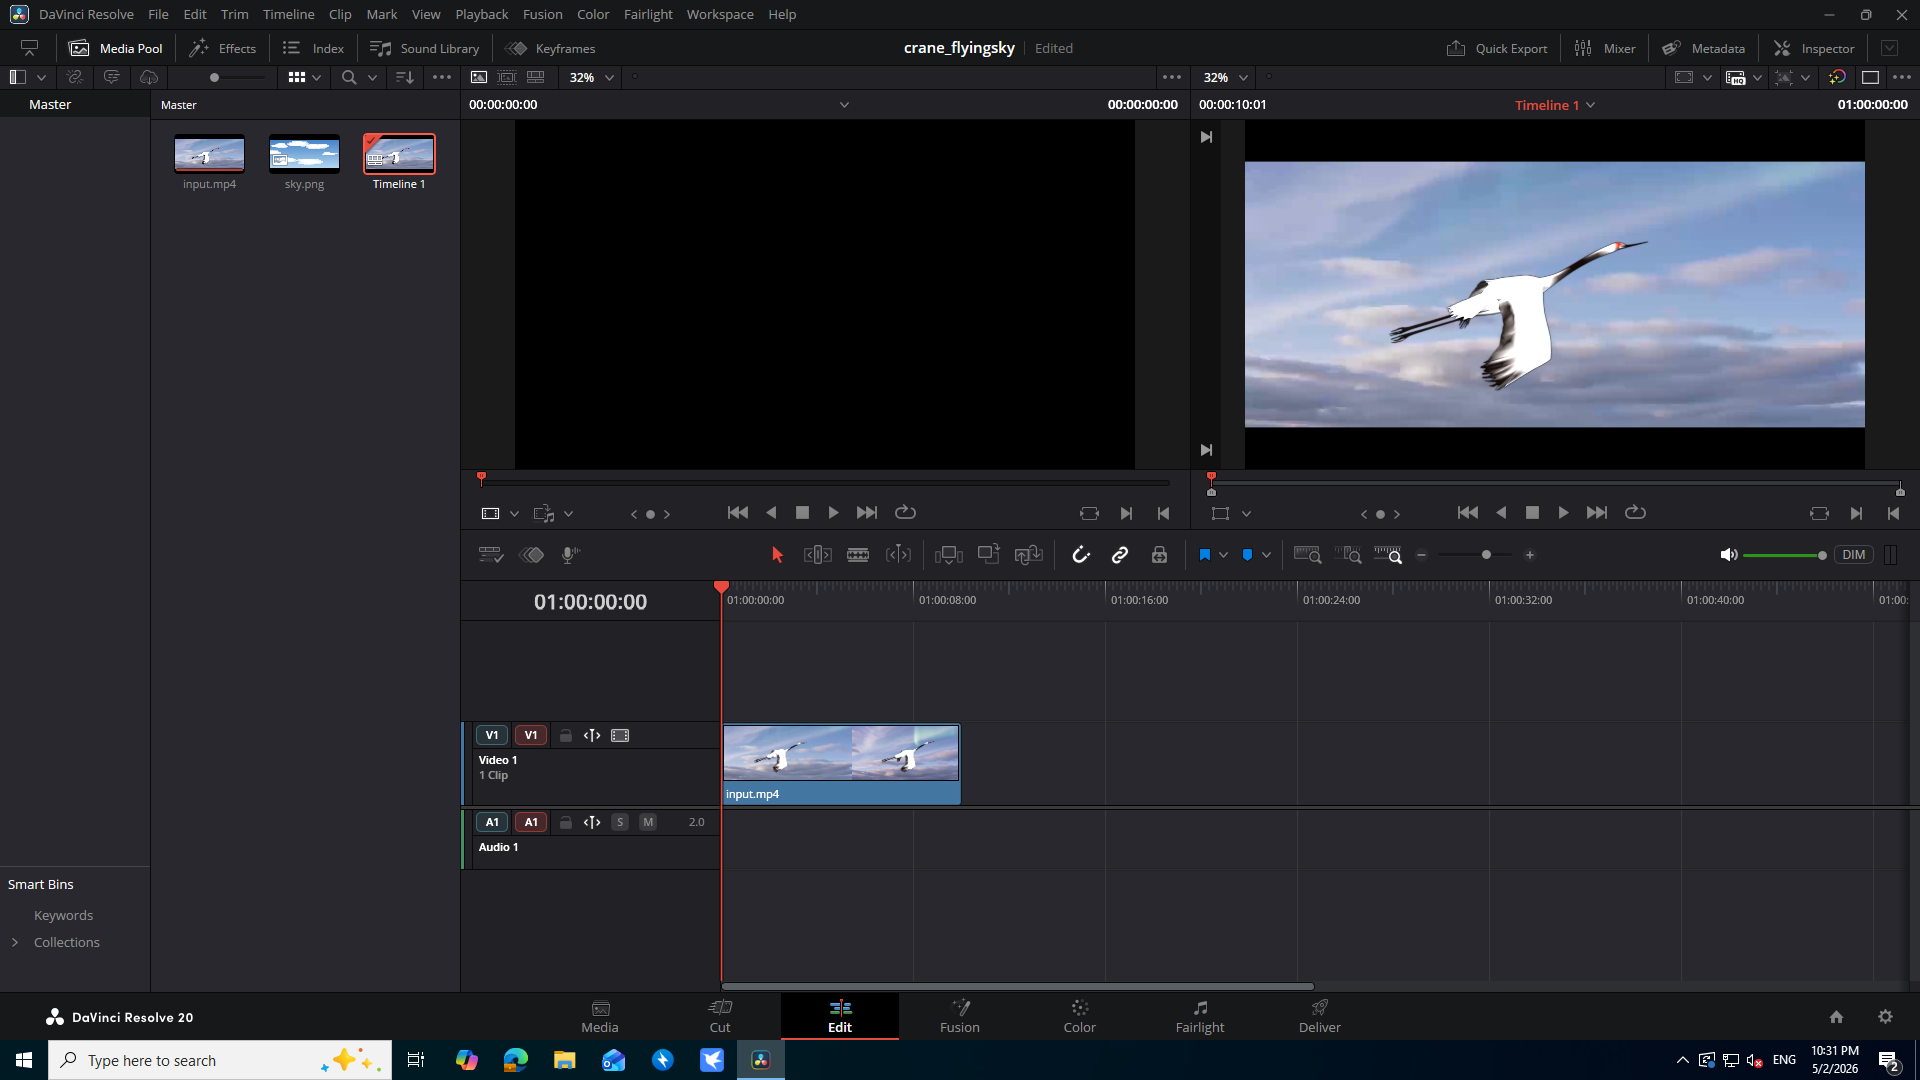
\includegraphics[width=0.985\linewidth,height=3.45in,keepaspectratio]{figures/task-card-assets/gui-economic/media-chroma-key-execution.png}

\vspace{1pt}
{\scriptsize VFX compositing workflow: DaVinci Resolve shows a timeline and preview monitor with the bird footage. The task required identifying the green-screen foreground, keying it, compositing it over the intended sky plate, and matching the reference frame.}
\end{CardBlock}

\begin{minipage}[t]{0.49\linewidth}
\vspace{0pt}
\begin{CardBlock}{inputbg}{inputbg}
\BlockTitle{INPUT MATERIALS}
\begin{itemize}
\item input.mp4 source clip for the keying workflow.
\item input.png reference frame defining target composition and foreground placement.
\item DaVinci Resolve desktop environment and required output path.
\end{itemize}
\end{CardBlock}

\begin{CardBlock}{inputbg}{inputbg}
\BlockTitle{REFERENCE OUTPUT}
\begin{itemize}
\item output/output.mp4 containing the composited bird shot.
\item Frames with foreground preserved, green screen removed, and contour/placement close to the reference.
\end{itemize}
\end{CardBlock}

\end{minipage}\hfill
\begin{minipage}[t]{0.49\linewidth}
\vspace{0pt}
\begin{CardBlock}{evalbg}{evalbg}
\BlockTitle{EVALUATION RUBRIC}
\begin{itemize}
\item Remote scoring samples frames from reference/breakpoint.json.
\item Foreground preservation is gated by roi\_input\_cv, and quality uses full-frame plus ROI edge IoU.
\item A local vision judge must also confirm that a real keying-related edit was made rather than a raw-source copy.
\end{itemize}
\end{CardBlock}

\begin{CardBlock}{analysisbg}{analysisbg}
\BlockTitle{OBSERVED OUTCOME}
\begin{itemize}
\item Score: 0.0. The agent used Resolve and exported an MP4, but the output did not satisfy the reference-based chroma-key transformation.
\item Failure mode: the submission treated a plausible bird-over-sky clip as the target instead of preserving the intended foreground/background relationship from the reference materials.
\item Interpretation: the error was in visual task grounding rather than software operation alone.
\end{itemize}
\end{CardBlock}
\end{minipage}
\end{ColorTaskCard}
\clearpage
\begin{ColorTaskCard}{Task Card 4: Skeletal Animation Reproduction \hfill \StatusBadge{PARTIAL}{partialbg}{partialorange}}
\scriptsize
{\textbf{Task ID:} \Code{game/skeletal_animation_reproduction}}\\[-1pt]
{\textbf{Observed score:} 0.429}\quad
\Chip{Game / 3D} \Chip{Blender} \Chip{Motion matching}

\begin{CardBlock}{summarybg}{summarybg}
\BlockTitle{TASK DESCRIPTION}
Animation production turns a static character asset into a rigged, replayable performance. The task provides a Blender environment, Singing.obj, and a reference motion video. The agent must rig the character, reproduce the body motion from reference.mp4, include 19 exact bone names, and submit both an editable final.blend and a replayable preview.mp4.
\end{CardBlock}

\begin{CardBlock}{softwarebg}{softwarebg}
\BlockTitle{SOFTWARE / EXECUTION VIEW}
\centering
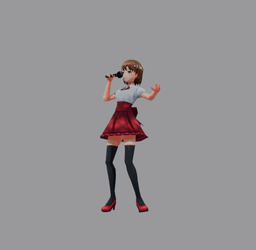
\includegraphics[width=0.985\linewidth,height=3.12in,keepaspectratio]{figures/task-card-assets/gui-economic/game-skeletal-animation-output.png}

\vspace{1pt}
{\scriptsize 3D animation output view: this render frame shows the rigged singer character from the agent's Blender submission. The task was to reproduce the body motion from a reference video, so a single valid-looking frame is only partial evidence; timing, pose range, and replay consistency determine success.}
\end{CardBlock}

\begin{minipage}[t]{0.49\linewidth}
\vspace{0pt}
\begin{CardBlock}{inputbg}{inputbg}
\BlockTitle{INPUT MATERIALS}
\begin{itemize}
\item Singing.obj static character mesh.
\item reference.mp4 body-motion target and reference/package.json bone-name requirements.
\item Blender runtime for rigging, keyframing, rendering, and replay validation.
\end{itemize}
\end{CardBlock}

\begin{CardBlock}{inputbg}{inputbg}
\BlockTitle{REFERENCE OUTPUT}
\begin{itemize}
\item final.blend containing a usable animated rig with the required bone names.
\item preview.mp4 whose body motion, timing, and pose range match the hidden clean reference.
\end{itemize}
\end{CardBlock}

\end{minipage}\hfill
\begin{minipage}[t]{0.49\linewidth}
\vspace{0pt}
\begin{CardBlock}{evalbg}{evalbg}
\BlockTitle{EVALUATION RUBRIC}
\begin{itemize}
\item Validity gates require both artifacts and a non-trivial animated rig.
\item Scoring combines video match, replay consistency from final.blend, minimal skeleton coverage, and binary vision checks.
\item Short or damped motion can lose credit even when the required files are present.
\end{itemize}
\end{CardBlock}

\begin{CardBlock}{analysisbg}{analysisbg}
\BlockTitle{OBSERVED OUTCOME}
\begin{itemize}
\item Score: 0.4285. The required Blender and preview artifacts existed and contained animation, so the run earned partial credit.
\item Failure mode: preview.mp4 was about 4 seconds while the reference was about 13.6 seconds, and the motion was damped to reduce mesh distortion.
\item Interpretation: the submission satisfied file-level validity but not the full motion-fidelity requirement.
\end{itemize}
\end{CardBlock}
\end{minipage}
\end{ColorTaskCard}
\clearpage
\begin{ColorTaskCard}{Task Card 5: MicroDicom Chest X-Ray Adjudication \hfill \StatusBadge{PARTIAL}{partialbg}{partialorange}}
\scriptsize
{\textbf{Task ID:} \Code{radiology/microdicom_nih_cxr_reader_adjudication}}\\[-1pt]
{\textbf{Observed score:} 0.333}\quad
\Chip{Radiology} \Chip{DICOM GUI} \Chip{Annotation QA}

\begin{CardBlock}{summarybg}{summarybg}
\BlockTitle{TASK DESCRIPTION}
Radiology dataset curation often requires adjudication between competing reader annotations. The task provides nine NIH CXR DICOM cases, two proposed atelectasis boxes per case, reader notes, and fixed TSV schemas. The agent must inspect each case in MicroDicom, choose the better reader annotation, and submit adjudicated\_boxes.tsv, adjudication\_log.tsv, and final\_impressions.tsv.
\end{CardBlock}

\begin{CardBlock}{softwarebg}{softwarebg}
\BlockTitle{SOFTWARE / EXECUTION VIEW}
\centering
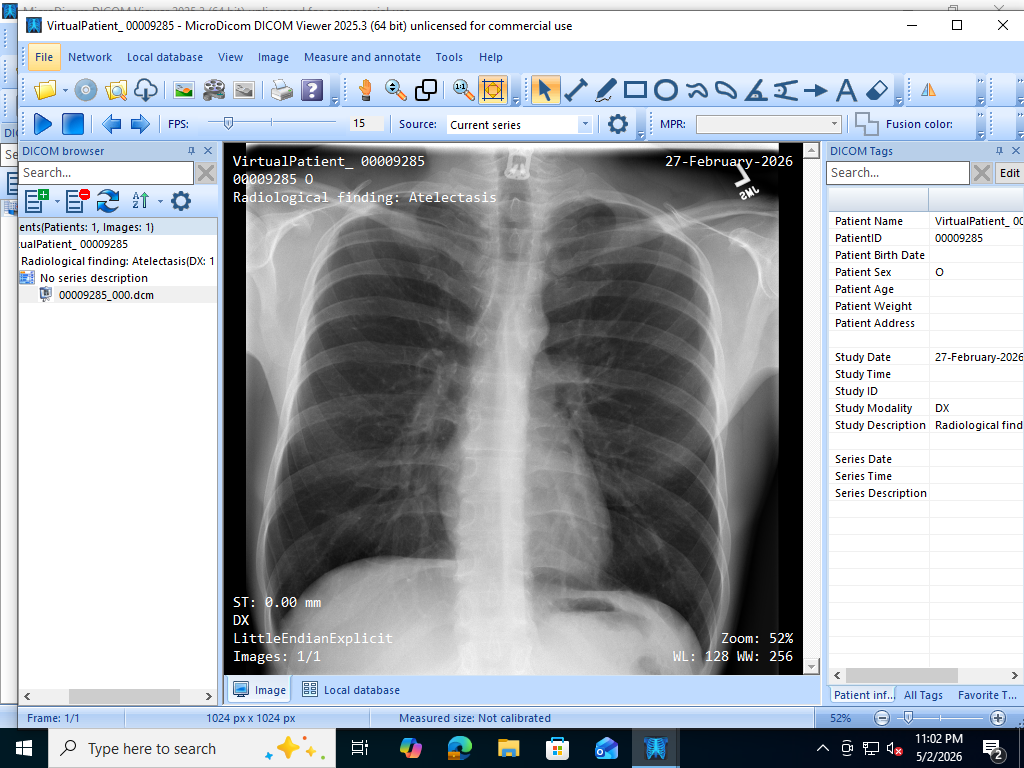
\includegraphics[width=0.985\linewidth,height=3.45in,keepaspectratio]{figures/task-card-assets/gui-economic/radiology-microdicom-execution.png}

\vspace{1pt}
{\scriptsize Radiology adjudication workflow: MicroDicom displays a chest X-ray with DICOM metadata and annotation tools. The task required reviewing each case, comparing two reader boxes for atelectasis, and writing TSV decisions; the deliverable depends on visual adjudication for each case.}
\end{CardBlock}

\begin{minipage}[t]{0.49\linewidth}
\vspace{0pt}
\begin{CardBlock}{inputbg}{inputbg}
\BlockTitle{INPUT MATERIALS}
\begin{itemize}
\item Nine DICOM chest X-ray cases with a case manifest.
\item reader\_a and reader\_b annotation TSVs plus clinical notes.
\item Rules fixing labels, allowed selected\_reader values, and output schemas.
\end{itemize}
\end{CardBlock}

\begin{CardBlock}{inputbg}{inputbg}
\BlockTitle{REFERENCE OUTPUT}
\begin{itemize}
\item adjudicated\_boxes.tsv with the final reader choice and box per case.
\item adjudication\_log.tsv and final\_impressions.tsv with the required rows and fixed labels.
\end{itemize}
\end{CardBlock}

\end{minipage}\hfill
\begin{minipage}[t]{0.49\linewidth}
\vspace{0pt}
\begin{CardBlock}{evalbg}{evalbg}
\BlockTitle{EVALUATION RUBRIC}
\begin{itemize}
\item Each TSV has hard gates for missing files, malformed headers, invalid reader values, or wrong fixed labels.
\item Log and impression files must match hidden references exactly by case\_id.
\item Box output must select the hidden-supported reader and achieve IoU at least 0.50 against the gold box.
\end{itemize}
\end{CardBlock}

\begin{CardBlock}{analysisbg}{analysisbg}
\BlockTitle{OBSERVED OUTCOME}
\begin{itemize}
\item Score: 0.3333. The agent wrote the three required TSV files covering all nine cases, but the score indicates only partial agreement with the hidden references.
\item Failure mode: detailed image review appears only for a few cases; later decisions relied on coordinates and heuristics rather than systematic visual adjudication.
\item Interpretation: file-format compliance was stronger than case-by-case visual-domain judgment.
\end{itemize}
\end{CardBlock}
\end{minipage}
\end{ColorTaskCard}
\clearpage
\endgroup
